\chapter{This is a chapter title}

..

\section{Accuracy results on island effects minimal pairs in Italian}

..

\subsection{Test description}

..

\subsection{Results table}

Results description: ..

The results are shown in \autoref{tab:accResults}.

% TODO: consider putting here only the values based on softmax, for less cols in the table. Add the full table to the appendix (in portait mode).
% TODO: use a smaller for for this table.

\begin{table} \scriptsize 
	\begin{center}
		\begin{tabular}{p{0.08\linewidth}|p{0.09\linewidth}|c|c|c|c|c|c|c|c|c|c|}
			  &  & \multicolumn{2}{c|}{Gpt2-it} & \multicolumn{4}{c|}{Bert-it}  & \multicolumn{4}{c|}{GilBERTo-it} \\
			 Pheno-menon & Sent. form & LP & PenLP & LP & PenLP & LP-L & PenLP-L & LP & PenLP & LP-L & PenLP-L \\
			\hline
			\multirow{3}{0.8cm}{Wh adjunct}  & Short-N.I. & \textbf{96} & 92 & 94 & 90 & \textbf{96} & \textbf{96} & 86 & 70 & 86 & 86 \\ 
				%	\cline{2-12}
		  			   & Long-N.I. & 98 & 86 & 66 & 40 & 60 & 58 & 64 & 34 & 4 & 4 \\ 
		  		%	   \cline{2-12}
		  			   & Short-I.S. & 96 & 98 & 100 & 98 & 100 & 100 & 94 & 94 & 84 & 88 \\ 
		  	\hline
		  	\multirow{3}{0.8cm}{Wh complex np} & Short-N.I. & 90 & 92 & 100 & 100 & 96 & 96 & 74 & 76 & 88 & 88 \\ 
		  			  		& Long-N.I. & 98 & 86 & 96 & 92 & 70 & 64 & 62 & 28 & 32 & 28 \\ 
		  					& Short-I.S. & 96 & 98 & 100 & 100 & 96 & 96 & 46 & 82 & 88 & 88 \\ 		  			 
		  	\hline
		  	\multirow{3}{0.8cm}{Wh subject} & Short-N.I. & 98 & 90 & 26 & 6 & 28 & 28 & 70 & 46 & 28 & 22 \\ 
		  	& Long-N.I. & 100 & 98 & 86 & 56 & 78 & 74 & 76 & 50 & 24 & 20 \\ 
		  	& Short-I.S. & 40 & 56 & 62 & 60 & 68 & 68 & 52 & 56 & 68 & 68 \\ 
		  	\hline
		  	\multirow{3}{0.8cm}{Wh whether} & Short-N.I. & 91.5 & 94.9 & 94 & 90 & 96 & 96 & 91.5 & 94.9 & 89.8 & 89.8 \\ 
		  	& Long-N.I. & 100 & 100 & 66 & 40 & 60 & 58 & 100 & 98.3 & 78 & 78 \\ 
		  	& Short-I.S. & 59.3 & 96.6 & 100 & 98 & 100 & 100 & 37.3 & 69.5 & 93.2 & 93 \\ 		  	
		\end{tabular}
		\caption{Accuracy results for Gpt-2 and Bert Italian models, on a testsuite of 50 items per phenomenon. The Gpt2-it model is LorenzoDeMattei/GePpeTto. The Bert-it model is dbmdz/bert-base-italian-xxl-cased. The GilBERTo-it model (an Italian RoBERTa variant) is idb-ita/gilberto-uncased-from-camembert.}
		\label{tab:accResults}
	\end{center}
\end{table}

..


\subsection{Italian models details}

Bert (dbmdz/bert-base-italian-xxl-cased): 81GB (13 billion tokens) of training data  and from Wikipedia, OPUS and OSCAR corpora. Model size 424 MB.
GePpeTto (LorenzoDeMattei/GePpeTto): 13.8GB of training data from Wikipedia and ItWac corpus. The model’s size corresponds to GPT-2 small, with 12 layers and 117M parameters. Vocab size 30k. 620k training steps.
GilBERTo (idb-ita/gilberto-uncased-from-camembert): Trained on ~71GB of Italian text (11.2 billion tokens) from the OSCAR corpus. Model size 420 MB


\section{Factorial test design}

..

\subsection{Introduction}

..

\subsection{Results}


É possibile riferire l'immagine, una volta assegnatagli una label, tramite il comando \texttt{\textbackslash autoref\{fig:immagine\}}, ottenendo il seguente risultato: \autoref{fig:immagine}.

\begin{figure}
	\centering
	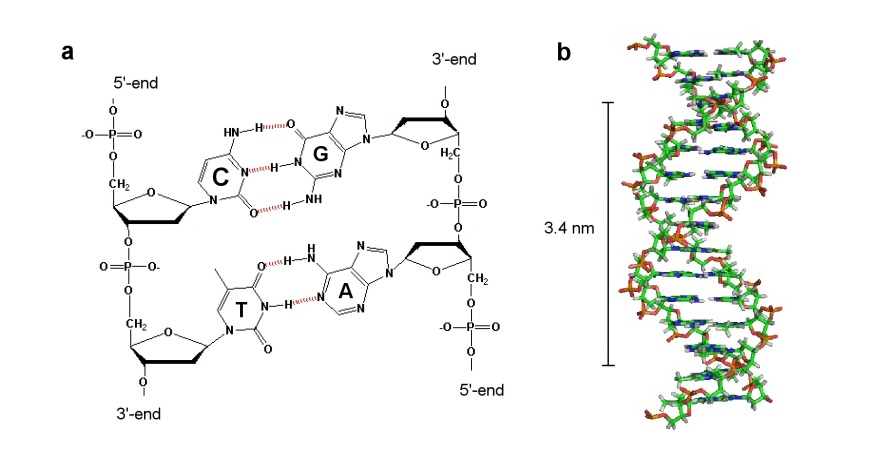
\includegraphics[width=0.8\textwidth]{images/Chapter1/immagine.jpg} % width= 0.8\textwidth
	\caption{This is an image} 
	\label{fig:immagine} % this internally labels the figure for future referencing.
\end{figure}

Fig.1 Results from Sprouse et al (2016)
Fig.2 Results of acceptability judgements to the same stimuli from Sprouse et al. 2016 from an Italian Gpt-2 model (GePpeTto) with the PenLP acceptability ..score. 
Fig.3

\subsection{Differences between the plots}

..
\subsubsection{Overall}
..
\subsubsection{Whether islands}
..
\subsubsection{Complex np islands}
..
\subsubsection{Subject islands}
..
\subsubsection{Adjunct islands}
..

\subsection{What seems to affect the models acceptability scores}
..
\subsubsection{Whether islands}
..
\subsubsection{Complex np islands}
..
\subsubsection{Subject islands}
..
\subsubsection{Adjunct islands}
..

\subsection{Future work}
..

\subsubsection{This is a sub-subsection}
..



Listing bibliography entries \citep{wei2021frequency, hu2020systematic, lau2020furiously,  sprouse2016experimental}

\subsubsection{This is another subsection}

Quello che segue è un esempio di codice. E' possibile modificare il linguaggio per il synyax highlight, aggiungere parole chiave... E' tutto disponibile nella guida del pacchetto \texttt{listings}.

\lstinputlisting[language=C++]{listings/Capitolo1/code1.cpp} 

\section{Blimp English dataset}
..
\subsection{English models details}
..

\section{Misc notes with refs}

“NATURAL LANGUAGE DOES NOT MAXIMIZE PROBABILITY” 
“Why is human-written text not the most probable text? We conjecture that this is an intrinsic property of human language. Language models that assign probabilities one word at a time without a global model of the text will have trouble capturing this effect. Grice’s Maxims of Communication (Grice, 1975) show that people optimize against stating the obvious. Thus, making every word as predictable as possible will be disfavored. This makes solving the problem simply by training larger models or improving neural architectures using standard per-word learning objectives unlikely: such models are forced to favor the lowest common denominator, rather than informative language.” 
\citep{holtzman2019curious}

Repeated exposure to a type of island construct will increase its perceived acceptability 
\citep{chaves2014subject}

Targed ..syntactic tests on modern language models seem to have started with \citet{linzen2016assessing}, while the use of psycholinguistic tests for this seem to have started with \citet{futrell2018rnns}.
